\documentclass[a4paper,10pt]{article}
\usepackage{caption}
\usepackage{cite}
\usepackage{mathtools}
\usepackage{pythonhighlight}
\usepackage{graphicx, subfigure}
\usepackage{hyperref}
\usepackage[english]{babel}
\usepackage[latin1]{inputenc}
%
\begin{document}
\captionsetup[figure]{labelfont={bf},name={Fig},labelsep=period}
%
   \title{Recognize MNIST database with RNN}

   \author{Lei Shiye}
          
   \date{2019\\ April}

   \maketitle
 
  \newpage
    
% This is a comment: in LaTeX everything that in a line comes
% after a "%" symbol is treated as comment
%\hypersetup{colorlinks=true, bookmarks, unicode}
\section*{Abstract}
% When adding * to \section, \subsection, etc... LaTeX will not assign
% a number to the section
For everyone who has learnt some knowledge of deep learning, he or she must be very familiar with using spatial convolutional neural network(\textbf{CNN}) or full-connected neural network(\textbf{FNN})to dealing with MNIST database. MNIST for deep learning is like "hello world!" for programme. When it comes to recurrent neural network(\textbf{RNN}), we always connect it to prediction problem like predicting tomorrow's weather through the weather of the last few days. How can we combine RNN with MNIST database? It is means that using RNN to solve MNIST recognition problem. In this report, I tried to construct a RNN architecture to recognize MNIST database and explain some confusions I have met in the process. 


\paragraph{Note:}
The source codes ralated to the report can be found on github:
\begin{verbatim} 
      https://github.com/LeavesLei/UPC-DL-lab-code/tree/master/lab_2/source_code_lab_2
\end{verbatim}

\section{Introduction}
\subsection{dataset}
The MNIST database is a large database of handwritten digits that is commonly used for training various image processing systems. The database is also widely used for training and testing in the field of machine learning. 

MNIST contains 60,000 training images and 10,000 testing images. All of images of MNIST are black and white and have same pixel of $28\times28$. Fig \ref{Fig.MNIST} has presented some cases in MNIST. 
\begin{figure}[htpb]
\centering 
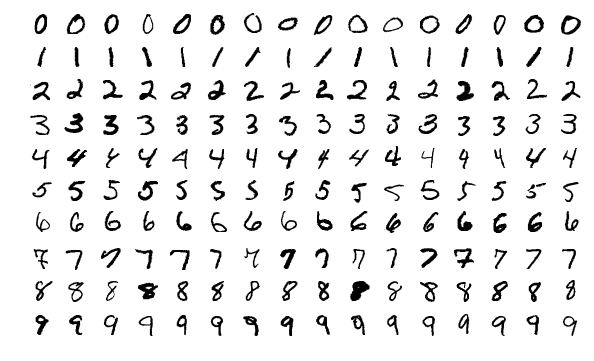
\includegraphics[width=1\textwidth]{report_image/mnist-all.png} 
\caption{MNIST} 
\label{Fig.MNIST} 
\end{figure}

\subsection{recurrent neural network}
When we talk about neural network, we will think of LeNet\cite{lecun1998gradient} or AlexNet\cite{krizhevsky2009learning}, which are famous CNN architecture and have a great effect in compute vision field. About RNN\cite{Elman90findingstructure}, Lost of people know of it. But the just know that RNN has a memory and no much else.

There is no doubt that humans or even lots of animals have memories. But how can machine remember things? The key is the hidden state. Every thing had happened will affect machine's hidden state. It's like that the machine talk to the things already happened that now that you make me a change so I will remember you.

\begin{figure}[htpb]
\centering 
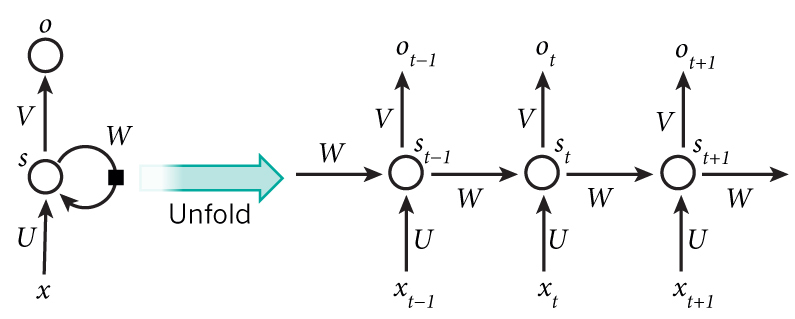
\includegraphics[width=1\textwidth]{report_image/rnn.jpg} 
\caption{basic RNN architecture} 
\label{Fig.RNN} 
\end{figure}

Fig \ref{Fig.RNN} present the basic architecture of recurrent neural network. Input $x$ is a vector of values for time t. $s_t$ is the hidden node at time $t$, which stores the state. One thing should be noticed that all weights($U, V, W$) are shared through time. Each step the computation uses the previous step, like below:

\[
s^{(t+1)}=f\left(s^{(t)}, x_{t+1} ; \theta\right)=f\left(f\left(s^{(t-1)}, x_{t} ; \theta\right), x_{t+1} ; \theta\right)=\cdots
\]
we can think of a RNN as a deep network that stacks layers through time.

Of course, activation functions are also used in RNN. The hyperbolic tangent function ($tanh$) is a popular
choice versus the usual $sigmoid$ function. Good results are also achieved using the rectified linear function ($ReLU$) instead. More computing details are as below:

\begin{equation}
    a^{(t)}=b+W \cdot s^{(t-1)}+U \cdot x^{(t)}
\end{equation}
\begin{equation}
    s^{(t)}=\tanh \left(a^{(t)}\right) 
\end{equation}
\begin{equation}
    y^{(t)}=c+V \cdot s^{(t)}
\end{equation}
$b$ and $c$ are bias, an additional step can be added depending on the task.

\section{Methods}
\subsection{Problem definition}
using RNN to recognize MNIST database is a strange problem. Should I use RNN to predict which number is the next one? Of course not. I will use RNN to recognize numbers that the images present in MNIST database. The key question is what format the input should be. The pixel of images in MNIST is $28\times28$. So we have two choice. The first one is convert an image to sequence with its length equals to $784$ and the input shape is $(784, 1)$. But its too redundancy. So I decided to convert an image to 28 row vectors and put them into RNN one by one. The input shape becames $(28, 28)$. And only take the last state as final output.

\subsection{RNN architecture}
I choose LSTM\cite{doi:10.1162/neco.1997.9.8.1735} as the basic RNN layer. After some tests, I thought 1 RNN layer is enough for this project with additional dense layer.
Fig \ref{Fig.mnist-rnn} is the neural network architecture in the experiment.
\begin{figure}[htpb]
\centering 
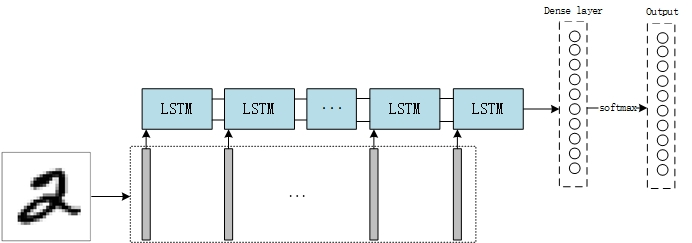
\includegraphics[width=1\textwidth]{report_image/mnist-rnn.jpg} 
\caption{architecture} 
\label{Fig.mnist-rnn} 
\end{figure}

\subsection{Parameter setting}
I want to train RNN model until it's overfitting. So I reduced the parameter neurons of LSTM constantly. When it decreased to 8, model become to show the phenomenon of overfitting. To solve overfitting, I set dropout to $0.5$ and had a good effect.
\begin{python}
    batch = 128
    epoch = 200
    optimizer = 'sgd'
    nlayers= 1     
    RNN = LSTM
    neurons = [4, 8, 16]
    drop = [0, 0.5]
    impl = 1
\end{python}

\section{Results}
I have run the code with $neurons=[4, 8, 16]$ and $dropout=[0, 0.5]$.

Fig \ref{Fig.accuracy-different neurons} showed the model accuracy with different number of neurons in LSTM unit. We can see that there is a higher accuracy and need fewer epoch to reach saturation with larger number of neurons. That's obvious. 

\begin{figure}[htpb] \centering    
\subfigure[neurons=4] {
 \label{fig:a}     
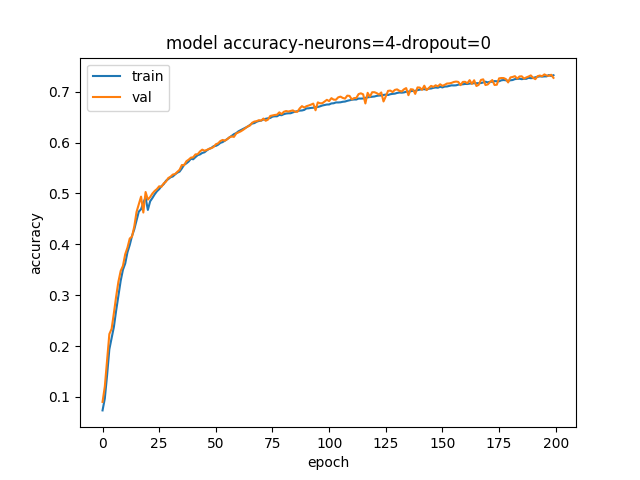
\includegraphics[width=0.3\columnwidth]{report_image/result/mnist_cnn_accuracy-neurons=4-dropout=0.png}  
}     
\subfigure[neurons=8] { 
\label{fig:b}     
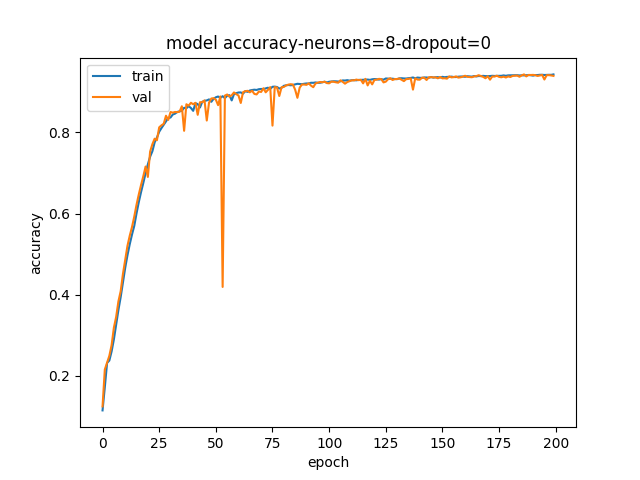
\includegraphics[width=0.3\columnwidth]{report_image/result/mnist_cnn_accuracy-neurons=8-dropout=0.png}     
}    
\subfigure[neurons=16] { 
\label{fig:c}     
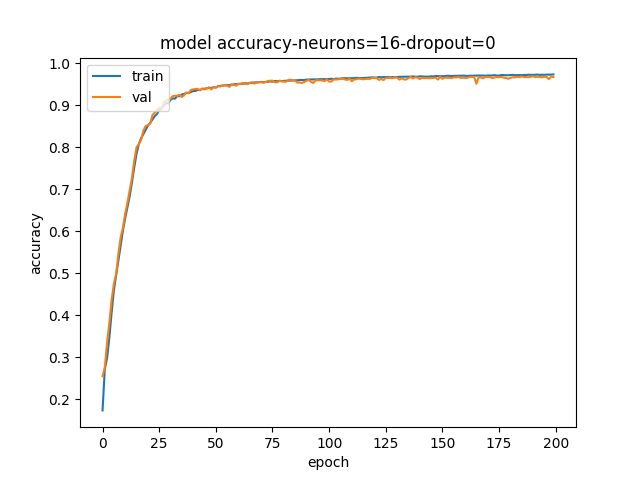
\includegraphics[width=0.3\columnwidth]{report_image/result/mnist_cnn_accuracy-neurons=16-dropout=0.png}     
}     
\caption{accuracy with different neurons}     
\label{Fig.accuracy-different neurons}     
\end{figure}    

Then I setted $dropout$ equals to $0.5$. I compared the result between $dropout=0$ and $dropout=0.5$ with the same number of $neurons=4$. The curves were presented in Fig \ref{Fig.accuracy-different dropout}
\begin{figure}[htpb] \centering    
\subfigure[dropout=0] {
 \label{fig:a}     
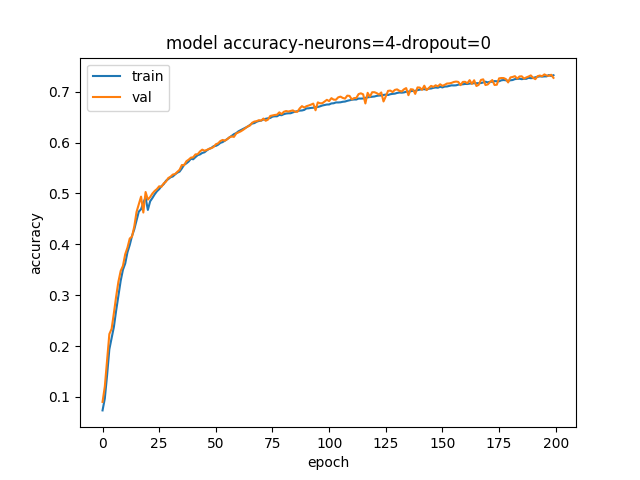
\includegraphics[width=0.45\columnwidth]{report_image/result/mnist_cnn_accuracy-neurons=4-dropout=0.png}  
}     
\subfigure[dropout=0.5] { 
\label{fig:b}     
\includegraphics[width=0.45\columnwidth]{report_image/result/{mnist_cnn_accuracy-neurons=4-dropout=0.5}.png}     
}       
\caption{accuracy with different dropout}     
\label{Fig.accuracy-different dropout}     
\end{figure}
We can draw something from the comparison that dropout can help speed the training speed and increase the accuracy.

I noticed that training curve and test curve in there images are very closed. It can be explained that out model with RNN has a good robustness and this raises a question for me: Does RNN architecture have a better generalization than basic CNN architecture? So I tried to recognize MNIST database with CNN. But CNN was so good that I cannot compare with them. I guess these reasons as below lead to higher generalization of RNN architecture:

   \begin{itemize}
      \item  RNN's three weight matrix: There are three weight matrix $W, V, U$. They are not order but dependent. It's like ensemble learning.
      \item  more input steps: RNN divide the input into several sections and deal with them step by step, which means more training samples. 
      \item  temporal architecture: RNN is a sequential neural network and like several layers architecture. It's more 'deeper' than basic CNN.
   \end{itemize}
   


\section{Discussion: softmax or sigmoid}
For a lot of machine learning beginners including me, they sometimes mix $sigmoid$ with $softmax$. When they felt confused, they will turn to reference books or Internet and found that $sigmoid=\frac{1}{{1+e^{-x}}}$ and $softmax=\frac{e^{x_j}}{\sum_{i=1}^{i=n}e^{x_i}}$. And they will forget it again soon. This is why we constantly study... 

Let's go down to business, I was thinking why $softmax$ is more frequently used in output layer then $sigmoid$? I begin to consider this question because I typed $softmax$ wrongly to $sigmoid$ when I wrote the code. When the training process begun, I found the optimization speed is slow.

I compared the results with using $sigmoid$ and $softmax$ in output layer, which is showed in Fig \ref{Fig.accuracy-different activation function}:

\begin{figure}[htpb] \centering    
\subfigure[sigmoid] {
 \label{fig:a}     
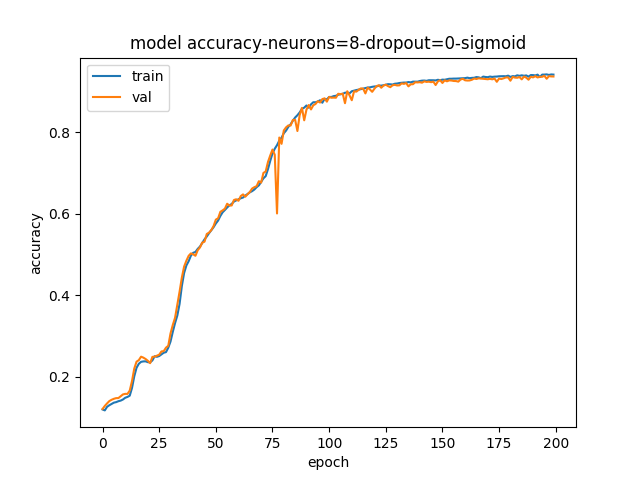
\includegraphics[width=0.45\columnwidth]{report_image/result/mnist_cnn_accuracy-neurons=8-dropout=0-sigmoid.png}  
}     
\subfigure[softmax] { 
\label{fig:b}     
\includegraphics[width=0.45\columnwidth]{report_image/result/{mnist_cnn_accuracy-neurons=8-dropout=0}.png}     
}       
\caption{accuracy with different activation function}     
\label{Fig.accuracy-different activation function}     
\end{figure}

It's apparent that training process is faster to reached saturation with $softmax$. So why is this happening? To figure out the question, I focused on their \textbf{back propagation process} first. 

I chose cross entropy as the loss function:
\[
CrossEntropy=-\frac{1}{n} \sum_{x}[y \ln a+(1-y) \ln (1-a)]
\] 
for example, the neural network is presented as Fig \ref{Fig.backpropagation}
\begin{figure}[htpb]
\centering 
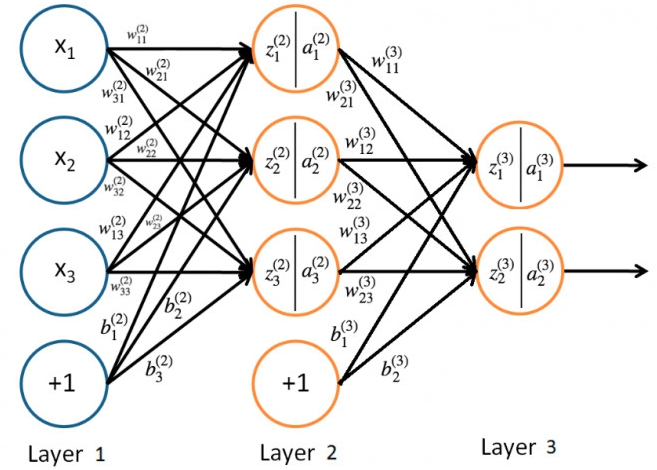
\includegraphics[width=1\textwidth]{report_image/backpropagation.jpg} 
\caption{neural network propagation} 
\label{Fig.backpropagation} 
\end{figure}

According to chain rule, the back propagation process can be presented as below:
\begin{equation*}
    \begin{split}
    \frac{\partial Loss}{\partial w^{(3)}} &= \frac{\partial Loss}{\partial a^{(3)}} \cdot \frac{\partial a^{(3)}}{\partial z^{(3)}} \cdot \frac{\partial z^{(3)}}{\partial w^{(3)}} \\
    &= \frac{\partial (-\frac{1}{n} \sum_{x}[y \ln a^{(3)}+(1-y) \ln (1-a^{(3)})])}{\partial a^{(3)}} \cdot \frac{\partial a^{(3)}}{\partial z^{(3)}} \cdot \frac{\partial a^{(2)} \cdot w^{(3)} + \cdots}{\partial w^{(3)}} \\
    &= -\frac{1}{n}\sum_{x}(\frac{y}{a^{(3)}}-\frac{1-y}{1-a^{(3)}}) \cdot \frac{\partial a^{(3)}}{\partial z^{(3)}} \cdot a^{(2)}
    \end{split}
\end{equation*}
So the key is to computing $\frac{\partial a^{(3)}}{\partial z^{(3)}}$

For $a^{(3)}=sigmoid(z^{(3)})=\frac{1}{1+e^{-a^{(3)}}}$:
\begin{equation*}
    \begin{split}
    \frac{\partial a^{(3)}}{\partial z^{(3)}} &= \frac{e^{-a^{(3)}}}{(1+e^{-a^(3)})^2} \\
    &= a^{(3)} \cdot (1-a^{(3)})
    \end{split}
\end{equation*}

For $a^{(3)}=softmax(z^{3})=\frac{e^{z_i^{(3)}}}{\sum e^{z^{(3)}}}$:

\begin{equation*}
    \begin{split}
    \frac{\partial a^{(3)}}{\partial z^{(3)}} &= \frac{e^{z_i^{(3)}} \cdot \sum e^{z^{(3)}} - e^{z_i^{(3)}} \cdot e^{z_i^{(3)}}}{\sum (e^{z^{(3)}})^2} \\
    &= \frac{e^{z_i^{(3)}}}{\sum e^{z^{(3)}}} - (\frac{e^{z_i^{(3)}}}{\sum e^{z^{(3)}}})^2 \\
    &= a^{(3)} \cdot (1-a^{(3)}) 
    \end{split}
\end{equation*}

It's same as $sigmoid$ !

so:
\begin{equation*}
    \begin{split}
    \frac{\partial Loss}{\partial w^{(3)}} &=  -\frac{1}{n}\sum_{x}(\frac{y}{a^{(3)}}-\frac{1-y}{1-a^{(3)}}) \cdot \frac{\partial a^{(3)}}{\partial z^{(3)}} \cdot a^{(2)} \\
    &= -\frac{1}{n}\sum_{x}(\frac{y}{a^{(3)}}-\frac{1-y}{1-a^{(3)}}) \cdot a^{(3)} \cdot (1-a^{(3)}) \cdot a^{(2)} \\
    &= -\frac{a^{(2)}}{n}\sum_{x}(y-a^{(3)})
    \end{split}
\end{equation*}

In general, I think there are two reasons for training speed more faster with $softmax$ than with $sigmoid$ as follows:

On the one hand, $sigmoid$ has a more strict remand with the output $z^{(3)}$. For instance, if the output is $z^{(3)} = [10, 5] $, so $a^{(3)}=sigmoid(z^{(3)})=[0.99995, 0.9933]$, which is not a good result. But if we used $softmax$ instead of $sigmoid$, $a^{(3)}=softmax(z^{(3)})=[0.9933, 0.0067]$, now we get a great prediction. so machine need more time for training more strict output with $sigmoid$.

On the other hands, machine can get more effective feedback with $softmax$. We have got the expression for gradient $\nabla=-\frac{a^{(2)}}{n}\sum_{x}(y-a^{(3)})$. when $z^{(3)}$ is small, even a huge negative, the gradient $\nabla$ will approximately equal to $0$. Or all of $z^{(3)}$ are large, the gradients $\nabla$ will approximately equal to $1$ and no difference between each other. If we changed activation function to $softmax$, we can get more different and efficient gradients which help us training models faster.

So this is why we always use $softmax$ for our activation function in output layer rather than $sigmoid$.


\section{Conclusions}
In the report, I tried to use RNN architecture to recognize MNIST database and increase the accuracy in various ways. Besides, the comparison of which activation function should be used in the output layer between $softmax$ and $sigmoid$ is discussed in detail in this report.


\newpage

\renewcommand\refname{Reference}
\bibliographystyle{plain}
\bibliography{ref}

\end{document}